\documentclass[11pt,a4paper]{article}

% =============================
% Packages
% =============================
\usepackage[margin=0.85in]{geometry}
\usepackage{setspace}
\usepackage{graphicx}
\usepackage{booktabs}
\usepackage{longtable}
\usepackage{tabularx}
\usepackage{array}
\usepackage{float}
\usepackage{xcolor}
\usepackage{fancyhdr}
\usepackage{titlesec}
\usepackage{caption}
\usepackage{hyperref}
\usepackage{wrapfig}
\usepackage{enumitem}
\usepackage{amsmath}

% =============================
% Document formatting
% =============================
\onehalfspacing
\hypersetup{colorlinks=true, linkcolor=black, urlcolor=blue}
\setlength{\parskip}{0.55em}
\setlength{\parindent}{0pt}
\renewcommand{\arraystretch}{1.18}
\newcolumntype{Y}{>{\raggedright\arraybackslash}X}

% =============================
% Section formatting
% =============================
\titleformat{\section}{\Large\bfseries}{\thesection}{0.7em}{}
\titleformat{\subsection}{\large\bfseries}{\thesubsection}{0.7em}{}

% =============================
% Footer/Header for subsequent pages
% =============================
\pagestyle{fancy}
\fancyhf{}
\fancyhead[L]{\today}
\fancyhead[R]{Generated by LAMBDA: \url{https://lambda.com.ai}}
\cfoot{\thepage}
\renewcommand{\headrulewidth}{0.4pt}

% =============================
% First page custom header
% =============================
\fancypagestyle{firstpage}{
    \fancyhf{}
    \fancyhead[L]{%
        Generated by LAMBDA: \url{https://lambda.com.ai}%
        \\[0.8em]
        \rule{\textwidth}{0.6pt}
    }
    \cfoot{\thepage}
    \renewcommand{\headrulewidth}{0pt}
}

\title{NAPH 10th Annual Report Analysis:\\Pulmonary Hypertension Care Quality\\in Great Britain (2018--19)}
\author{LAMBDA}
\date{\today}

\begin{document}
\thispagestyle{firstpage}

\begin{center}
  \vspace*{3cm}
  {\LARGE \textbf{NAPH 10th Annual Report Analysis}} \\[0.5em]
  {\Large Pulmonary Hypertension Care Quality} \\[0.3em]
  {\Large in Great Britain (2018--19)} \\[1em]
  {\large LAMBDA} \\[0.5em]
  {\large \today}
\end{center}

\vfill

\begin{abstract}
\noindent This report analyses data from the 10th National Audit of Pulmonary Hypertension (NAPH), covering care quality across eight specialist PH centres in Great Britain during 2018--19. The analysis synthesises national standards performance, centre-level variation, local action plans from five centres, and Kaplan-Meier survival curves for idiopathic pulmonary arterial hypertension (IPAH) patients stratified by sex, age, and WHO functional class. Key findings include: 11 of 13 national standards were met at aggregate level; survival is strongly predicted by age quintile and comorbidity status (48\% five-year survival for young women without comorbidities versus 25\% for older patients with comorbidities); pulmonary endarterectomy waiting times remain the single largest quality gap at 11\% compliance against a 90\% target; and local action plan coverage is narrow, addressing primarily Standards 3, 5, 8, and 13. Scottish patient data are excluded from survival analysis due to pseudo-nymisation constraints.
\end{abstract}

\newpage

\tableofcontents
\newpage

\section{What matters most}

Eleven of 13 national standards were met at a national level, demonstrating overall high-quality care delivery across specialist PH centres. The two major gaps are Standard 7 (vasoreactivity study recording: 57\% vs.\ 80\% target) and Standard 13 (PEA waiting times: only 11\% vs.\ 90\% target). Survival for IPAH patients is strongly predicted by age, sex, and WHO functional class: younger women without comorbidities achieve approximately 80\% five-year survival, while older men with comorbidities drop below 40\% within three years. Pulmonary endarterectomy (PEA) waiting times represent the single largest quality gap -- only 11\% of cases meet the four-month standard nationally, and no individual centre exceeded 23\%. Drug therapy initiation timing has stagnated around 81\%, just barely above the 80\% target, with Sheffield declining from 87\% to 79\%. Local action plan coverage is narrowly focused, with only four distinct standards addressed across five submitted documents.

\section{Patient populations and survival outcomes}

The longitudinal cohort tracks adult patients whose first referral was on or after 1 April 2009, providing 23,311 patient records spanning ten years of prospective data collection. Across this cohort, cumulative survival drops steadily from 85\% at one year post-diagnosis, through 75\% at two years, 60\% at three years, 50\% at four years, and 45\% at five years. By definition, the survival curves are stopped when the remaining patient count falls below 50, so longer-term estimates carry wider uncertainty and should be interpreted as lower bounds.

\subsection{Overall cohort survival}

Figure~\ref{fig:survival_sex} presents Kaplan--Meier survival curves stratified by sex and comorbidity status for IPAH patients. Female patients without comorbidities demonstrate superior long-term survival, reaching 48\% at eight years. Male patients with comorbidities experience the steepest decline, reaching 40\% by approximately three years. The curve for males without comorbidities falls between these extremes at 36\% by six years.

\begin{figure}[H]
  \centering
  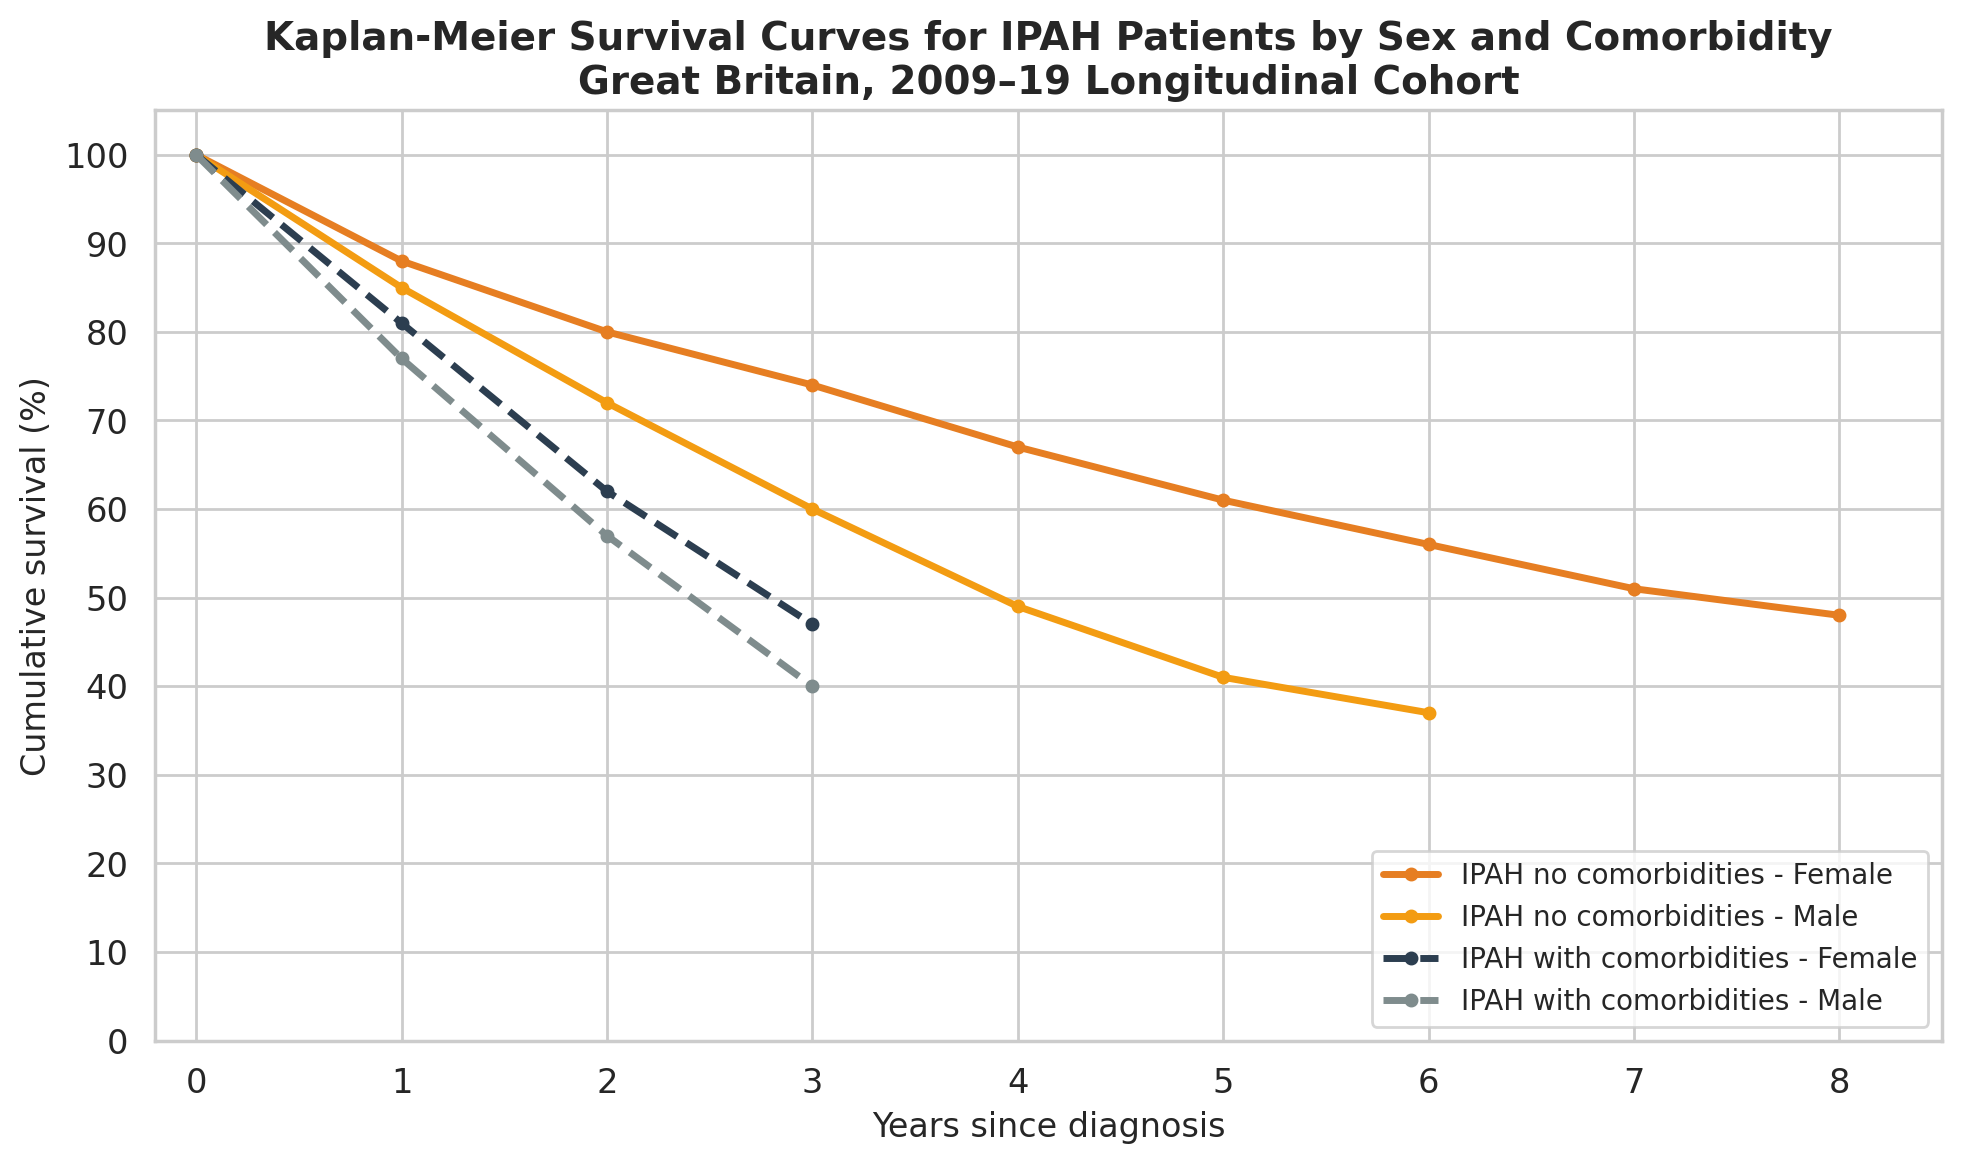
\includegraphics[width=\textwidth]{survival_by_sex.png}
  \caption{Kaplan--Meier survival curves for IPAH patients stratified by sex and comorbidity status. Female patients without comorbidities demonstrate superior long-term survival (approximately 48\% at eight years), while males with comorbidities experience the steepest decline (approximately 40\% at three years).}
  \label{fig:survival_sex}
\end{figure}

\subsection{Sex differences in survival}

The most pronounced survival disparity exists between women and men with IPAH without comorbidities. Women diagnosed in this group maintain an average of seven years and seventy-seven days to reach median mortality, compared to just three years and two hundred and seventy-nine days for men -- a difference of roughly four years. 

These results are striking because baseline haemodynamic parameters are remarkably similar across sexes. Mean pulmonary artery pressure averages 52.3 mmHg for women and 49.2 mmHg for men. WHO functional class III represents 71\% of women versus 74\% of men. Mixed venous oxygen saturation, cardiac index, and transfer factor for carbon monoxide are nearly identical. The prognosis differential therefore does not appear to arise from more severe disease presentation among men.

Patients with comorbidities face dramatically worse survival regardless of sex. For women with comorbid IPAH, cumulative survival reaches 40\% by 3.5 years; for men with comorbid IPAH, it reaches 40\% by 3 years. The presence of additional cardiac or respiratory disease nearly halves expected survival time. Median age at diagnosis among women with comorbidities is 69 years, compared to 57 years for those without.

\subsection{Age quintiles reveal steep gradients}

Age at diagnosis is perhaps the strongest predictor of survival trajectory. Five age-based quintiles show monotonic declines across all follow-up intervals:

\begin{table}[H]
\centering
\small
\caption{Survival by age quintile for IPAH patients without comorbidities}
\begin{tabularx}{\textwidth}{lccccY}
\toprule
Quintile & Age Range & Median Age (\%) Female & 3-Year Survival & 5-Year Survival & Days to 50\% Mortality \\
\midrule
Q1 & 18--41 & 32 (76\%) & 90\% & 84\% & Not reached at 6+ years \\
Q2 & 41--54 & 47 (72\%) & 85\% & 75\% & Not reached at 6+ years \\
Q3 & 54--66 & 60 (64\%) & 70\% & 46\% & 4 years + 127 days \\
Q4 & 66--74 & 70 (56\%) & 55\% & -- & 3 years + 203 days \\
Q5 & 74--91 & 78 (59\%) & 46\% & -- & 2 years + 291 days \\
Comorbidities (all ages) & 26--90 & -- & 43\% & 25\% & 2 years + 218 days \\
\bottomrule
\end{tabularx}
\end{table}

The progression from Q1 to Q5 shows that each five-year increment in median age at diagnosis reduces five-year survival by approximately 10 percentage points within the ``no comorbidities'' population. Patients in the youngest quintile (Q1, median age 32) maintain 84\% survival at five years. By contrast, patients with comorbidities -- who span all age ranges but tend toward older diagnoses (median age 70) -- drop to 25\% survival at five years.

The female representation rate declines with age among patients without comorbidities: from 76\% in Q1 down to 56\% in Q4. This may partly reflect changing epidemiology across decades of referral data.

\begin{figure}[H]
  \centering
  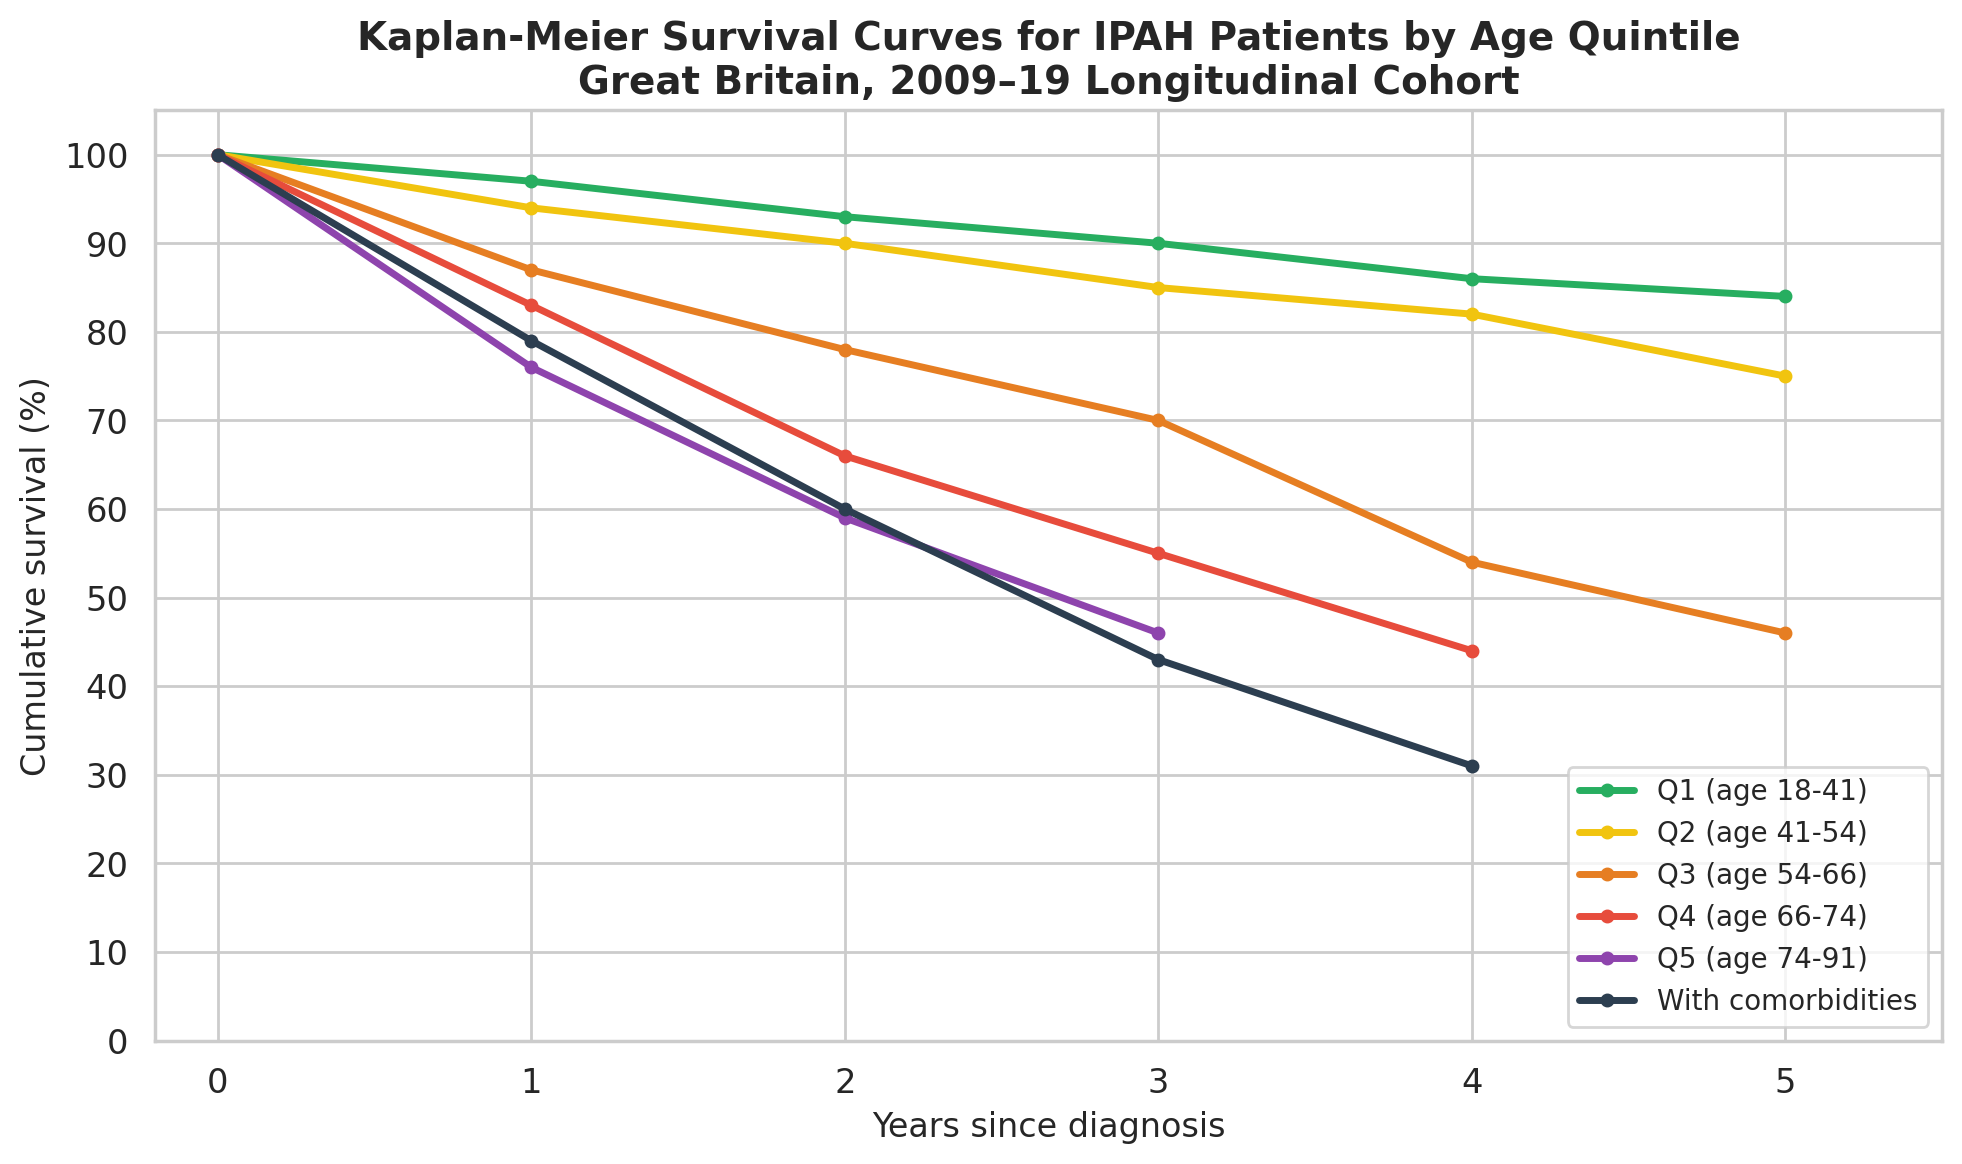
\includegraphics[width=\textwidth]{survival_by_age.png}
  \caption{Survival curves across five age quintiles show a clear dose-response relationship between age at diagnosis and mortality risk. The comorbidities group (combining all quintiles, $n = 77$) consistently underperforms even the oldest age-only quintile.}
  \label{fig:survival_age}
\end{figure}

\subsection{WHO functional class predicts near-term outcomes}

Among patients with IPAH without comorbidities, WHO functional class at diagnosis provides the best short-term prognostic signal:

\begin{itemize}[leftmargin=*, nosep]
    \item \textbf{WHO class II}: 80\% survive to 3 years, with data extending to approximately 4 years where survival remains at 75\%. Only 103 patients initiated in this category, limiting longer-term estimates.
    \item \textbf{WHO class III}: The largest group (811 patients), showing 72\% survival at 3 years, dropping to 43\% by 8 years.
    \item \textbf{WHO class IV}: Despite being the most severely symptomatic group (213 patients), 55\% survive to 3 years, with 48\% at 4 years -- better than some might expect, suggesting that severe presentations often lead to aggressive treatment.
\end{itemize}

For patients with comorbidities, WHO class III shows 50\% survival at 3 years, falling to 34\% by 4 years. WHO class IV with comorbidities lacks sufficient sample size (only 106 patients) to sustain meaningful survival estimates beyond 2 years, stopping at approximately 55\% at that point.

\begin{figure}[H]
  \centering
  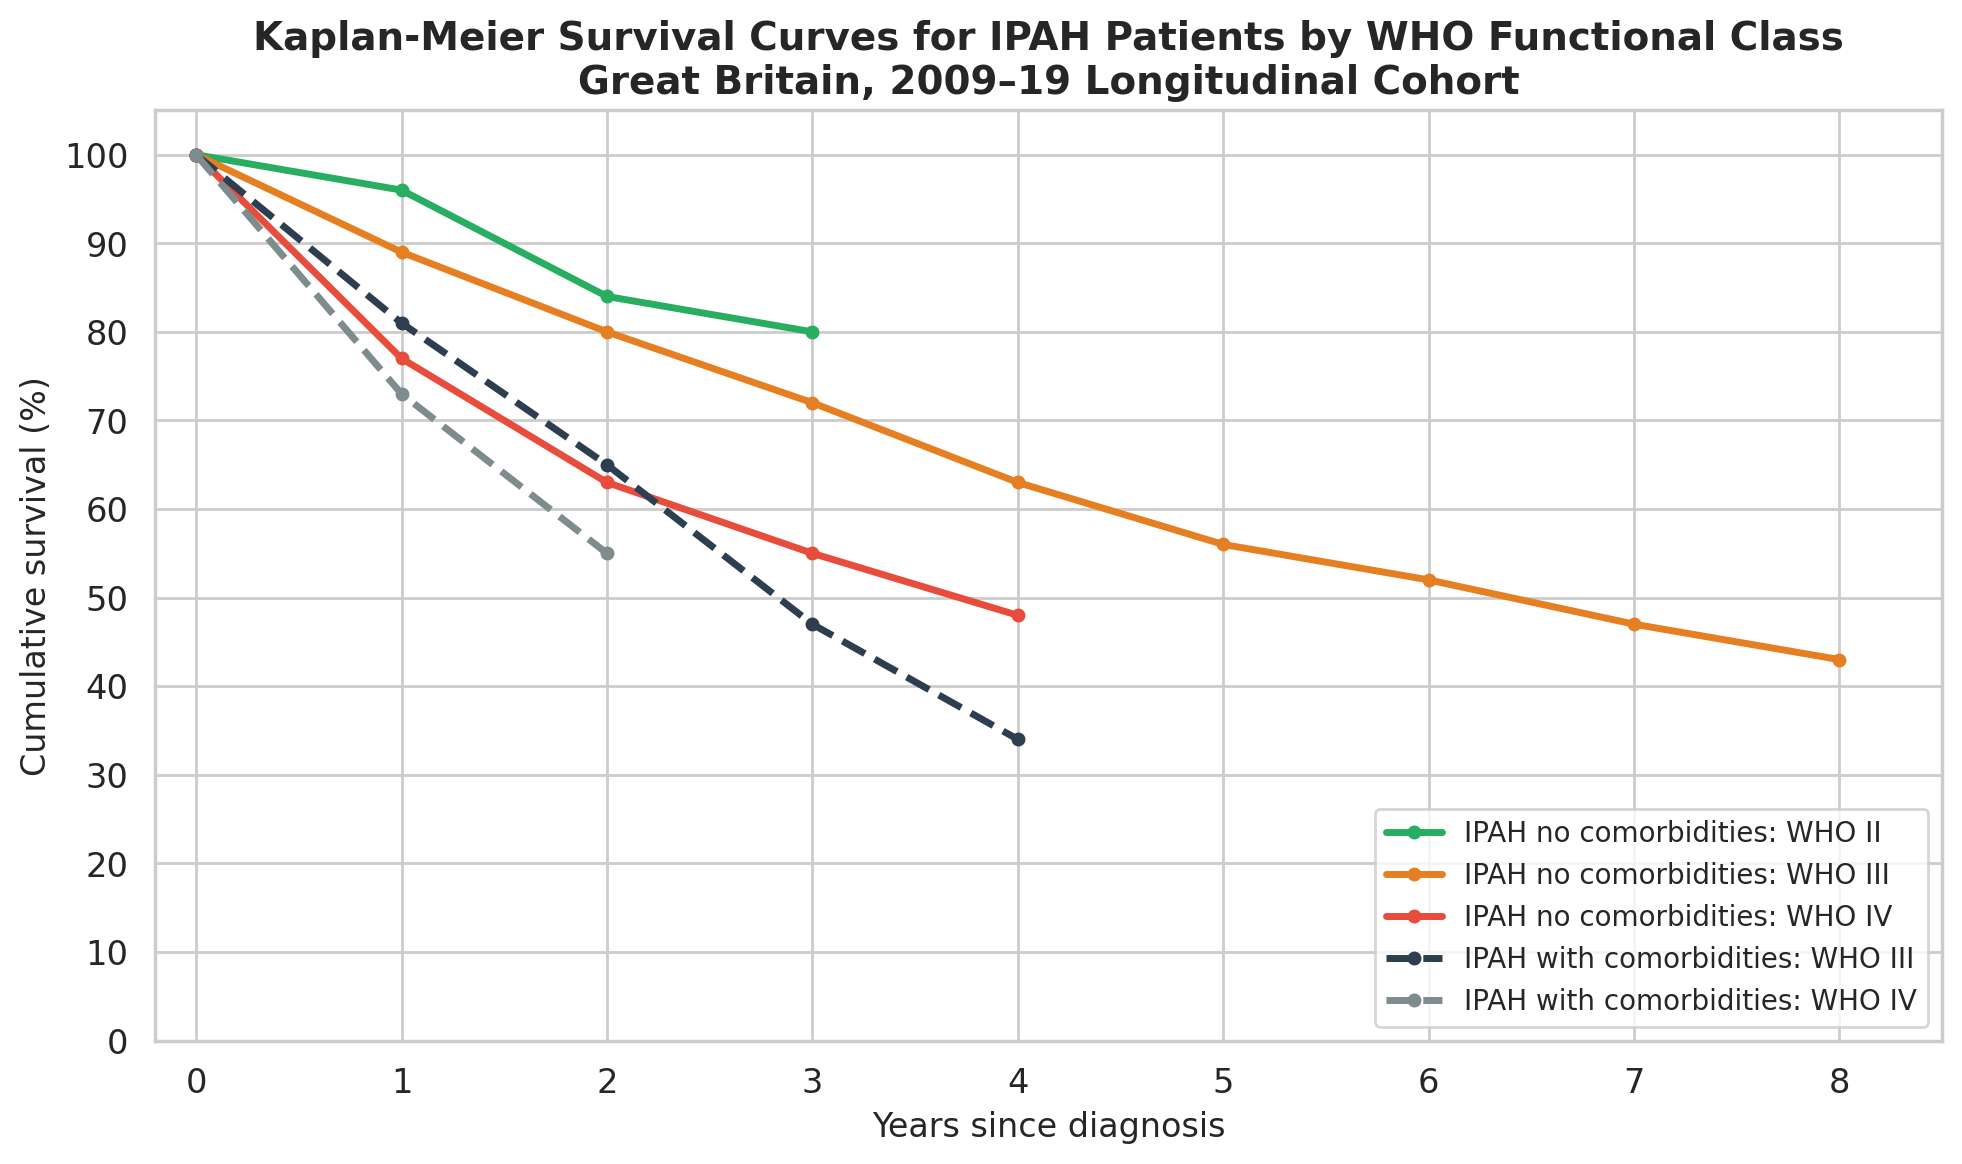
\includegraphics[width=\textwidth]{survival_by_who_class.png}
  \caption{WHO functional class at diagnosis clearly stratifies patients by medium-term survival, with class II outperforming class III by approximately 20 percentage points at three years. Comorbidity groups consistently underperform their age-matched counterparts.}
  \label{fig:survival_who}
\end{figure}

\section{National standards performance: trends and gaps}

At a national aggregate level, the audit demonstrates strong performance across most clinical indicators. Table~\ref{tab:national_standards} summarises trends from 2015--16 through 2018--19.

\begin{table}[H]
\centering
\resizebox{\textwidth}{!}{%
\begin{tabular}{lcrrrrrY}
\toprule
Standard & Description & Target & 2015--16 & 2016--17 & 2017--18 & 2018--19 & Trend & Status \\
\midrule
NS 1 & Centre participation & All centres & 7/8 & 8/8 & 8/8 & 8/8 & Steady & Met \\
NS 2 & Sufficient caseload $\geq$300 pts & 300 & 7/7 & 8/8 & 8/8 & 8/8 & Steady & Met \\
NS 3 & Timely diagnosis & 95\% & 96\% & 98\% & 98\% & 99\% & Up & Met \\
NS 4 & Seen within 30 days & 50\% & 47\% & 53\% & 60\% & 63\% & Up & Met \\
NS 5 & Cardiac cath before treatment & 95\% & 91\% & 96\% & 96\% & 97\% & Steady & Met \\
NS 6 & WHO class \& exercise test & 90\% & 80\% & 85\% & 98\% & 97\% & Steady & Met \\
NS 7 & Vasoreactivity study & 80\% & -- & -- & -- & 57\% & New & Not met \\
NS 8 & Drug therapy $<$12 weeks & 80\% & 76\% & 82\% & 81\% & 81\% & Steady & Met \\
NS 9 & Diagnosis on drug record & 99\% & 100\% & 100\% & 100\% & 100\% & Steady & Met \\
NS 10 & PDE5 first-line therapy & 80\% & 90\% & 92\% & 93\% & 91\% & Steady & Met \\
NS 11 & Quality of life recorded & 90\% & 78\% & 89\% & 96\% & 96\% & Steady & Met \\
NS 12 & Annual consultation & 90\% & 96\% & 96\% & 96\% & 96\% & Steady & Met \\
NS 13 & PEA wait $<$4 months & 90\% & 14\% & 13\% & 18\% & 11\% & Steady & Not met \\
\bottomrule
\end{tabular}%
}
\caption{National Standards performance across four audit years. NS 7 (vasoreactivity study) is newly introduced. NS 13 (PEA waiting times) remains the most persistent outlier.}
\label{tab:national_standards}
\end{table}

Several noteworthy patterns emerge from this timeline:

\begin{itemize}[nosep]
    \item \textbf{NS 6 (WHO class and exercise test)} improved dramatically from 80\% in 2015--16 to 98\% in 2017--18, then plateaued. Documentation discipline appears largely established.
    \item \textbf{NS 4 (Seen within 30 days)} climbed consistently from 47\% to 63\%, achieving the milestone of 100\% of centres meeting their respective targets in 2018--19 for the first time. Newcastle improved from 19\% to 78\%.
    \item \textbf{NS 11 (Quality of life recorded)} doubled its rate from 78\% to 96\% within three years, reflecting improved integration of emPHasis-10 scoring into routine clinical workflows.
    \item \textbf{NS 13 (PEA waiting times)} has fluctuated between 11\% and 18\% with no sustained improvement. The median time from diagnosis to PEA surgery has shortened since 2016, yet structural constraints continue to keep performance far below the 90\% target.
    \item \textbf{NS 8 (Drug therapy within 12 weeks)} rose from 76\% to 82\% initially, then settled back to 81\%, hovering barely above the 80\% floor. Sheffield declined from 87\% to 79\%.
\end{itemize}

\begin{figure}[H]
  \centering
  
\includegraphics[width=\textwidth]{national_standards_timeline.png}
  \caption{National Standards performance across four audit years. Green bars indicate targets were met; red indicates failure to meet targets; grey indicates not applicable (e.g., NS 7 was newly introduced in 2018--19). NS 13 remains the most persistent outlier.}
  \label{fig:standards_timeline}
\end{figure}

\subsection{Centre-level variation}

Performance against national standards varies meaningfully between centres. In 2018--19, no centre failed every standard, but every centre missed at least one:

\begin{table}[H]
\centering
\resizebox{\textwidth}{!}{%
\scriptsize
\begin{tabular}{lccccccccc}
\toprule
Standard & Target & Golden Jubilee & GOS & Imperial & Newcastle & Royal Brompton & Royal Free & Royal Papworth & Sheffield \\
\midrule
NS 3 & 95\% & \textcolor{green}{99\%} & \textcolor{red}{89\%} & \textcolor{green}{100\%} & \textcolor{red}{94\%} & \textcolor{green}{99\%} & \textcolor{green}{99\%} & \textcolor{green}{99\%} & \textcolor{green}{100\%} \\
NS 4 & 50\% & \textcolor{green}{74\%} & \textcolor{green}{100\%} & \textcolor{green}{62\%} & \textcolor{green}{78\%} & \textcolor{green}{57\%} & \textcolor{green}{75\%} & \textcolor{green}{53\%} & \textcolor{green}{55\%} \\
NS 5 & 95\% & \textcolor{green}{99\%} & N/A & \textcolor{red}{92\%} & \textcolor{green}{100\%} & \textcolor{green}{97\%} & \textcolor{green}{97\%} & \textcolor{green}{97\%} & \textcolor{green}{98\%} \\
NS 6 & 90\% & \textcolor{green}{100\%} & N/A & \textcolor{green}{92\%} & \textcolor{green}{94\%} & \textcolor{green}{96\%} & \textcolor{green}{97\%} & \textcolor{green}{94\%} & \textcolor{green}{98\%} \\
NS 8 & 80\% & \textcolor{red}{61\%} & N/A & \textcolor{green}{89\%} & \textcolor{green}{91\%} & \textcolor{green}{88\%} & \textcolor{green}{87\%} & \textcolor{red}{75\%} & \textcolor{red}{79\%} \\
NS 10 & 80\% & \textcolor{green}{89\%} & N/A & \textcolor{green}{100\%} & \textcolor{red}{86\%} & \textcolor{red}{84\%} & \textcolor{green}{95\%} & \textcolor{green}{96\%} & \textcolor{green}{91\%} \\
NS 11 & 90\% & \textcolor{green}{94\%} & N/A & \textcolor{green}{95\%} & \textcolor{green}{100\%} & \textcolor{green}{93\%} & \textcolor{green}{98\%} & \textcolor{green}{93\%} & \textcolor{green}{99\%} \\
NS 13 & 90\% & 23\% & N/A & 10\% & 0\% & 0\% & 0\% & 23\% & 6\% \\
\bottomrule
\end{tabular}%
}
\caption{Centre-level performance against National Standards (2018--19). Green indicates target met; red indicates target not met. Royal Papworth Hospital serves as the national PEA centre and is the only centre with substantial PEA-related referrals.}
\label{tab:centre_performance}
\end{table}

Royal Papworth Hospital, the national PEA centre, achieved 23\% compliance with Standard 13 -- tied with Golden Jubilee for the highest rate among centres reporting this metric. However, Royal Papworth also scored lowest at 75\% on Standard 8 (drug therapy within 12 weeks), confirming that its high volume of diagnostic assessments creates bottlenecks elsewhere in the pathway.

Three centres -- Newcastle, Royal Brompton, and Royal Free -- achieved 0\% on Standard 13 because they do not perform PEA themselves and refer all such patients to Royal Papworth. These centres track local delays but cannot control surgical scheduling directly.

Golden Jubilee's 61\% on Standard 8 is the lowest non-N/A result in that row, consistent with their stated bottleneck in right heart catheterisation throughput. Imperial College's 92\% on NS 5 falls just below the 95\% target, though documentation reviews suggest many catheterizations were performed externally and not captured.

\begin{figure}[H]
  \centering
  
\includegraphics[width=\textwidth]{centre_comparison_2018_19.png}
  \caption{PH centre performance against selected National Standards in 2018--19. Colour coding matches the summary tables: green for targets met, red for unmet. Royal Papworth's dual role as both diagnostic centre and national PEA centre creates trade-offs visible in the divergent NS 8 and NS 13 scores.}
  \label{fig:centre_comparison}
\end{figure}

\subsection{The PEA waiting time crisis}

National Standard 13 deserves separate attention. Only 11\% of cases met the four-month waiting time target in 2018--19, representing a 79-percentage-point gap from the 90\% target. Performance fluctuates modestly over four audit cycles (14\% $\to$ 13\% $\to$ 18\% $\to$ 11\%) but never approaches the threshold.

\begin{figure}[H]
  \centering
  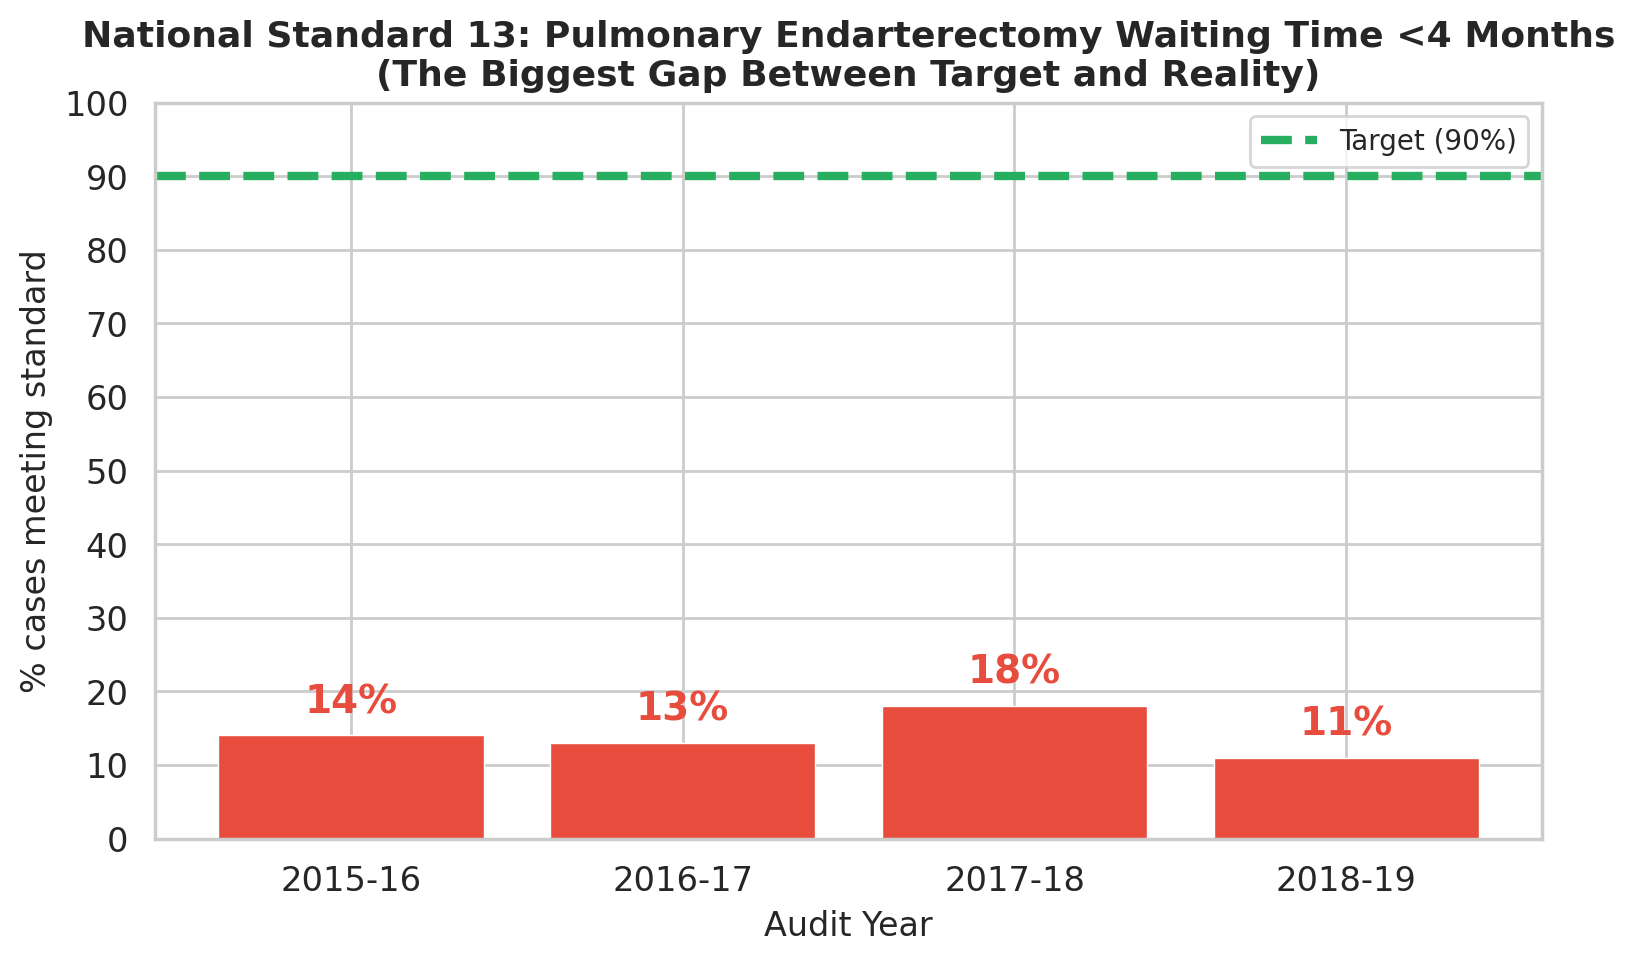
\includegraphics[width=0.65\textwidth]{ns13_pea_gap.png}
  \caption{National Standard 13 performance over four years remains below 20\%, with a 79-percentage-point gap from the 90\% target. The dashed green line marks the target level.}
  \label{fig:pea_gap}
\end{figure}

Kathy Blacker, Lead Commissioner for NHS England, acknowledges the multifactorial nature of these delays: ``The median time from diagnosis to PEA surgery has improved since 2016 but unfortunately the majority of patients still do not meet standard 13.'' The commissioners and PH centres have committed to pathway meetings and planning for increasing surgical capacity at Royal Papworth.

\section{Local Action Plan analysis}

Five of the eight specialist PH centres submitted Local Action Plan documents for the 10th Annual Report: Sheffield, Royal Brompton, Newcastle, Imperial College, and Golden Jubilee. Great Ormond Street (children's centre), Imperial College (for NS 13), and Newcastle (for NS 13) cross-referenced Royal Papworth's response rather than submitting centre-specific actions for PEA-related delays. Together, these documents address four distinct national standards.

\begin{figure}[H]
  \centering
  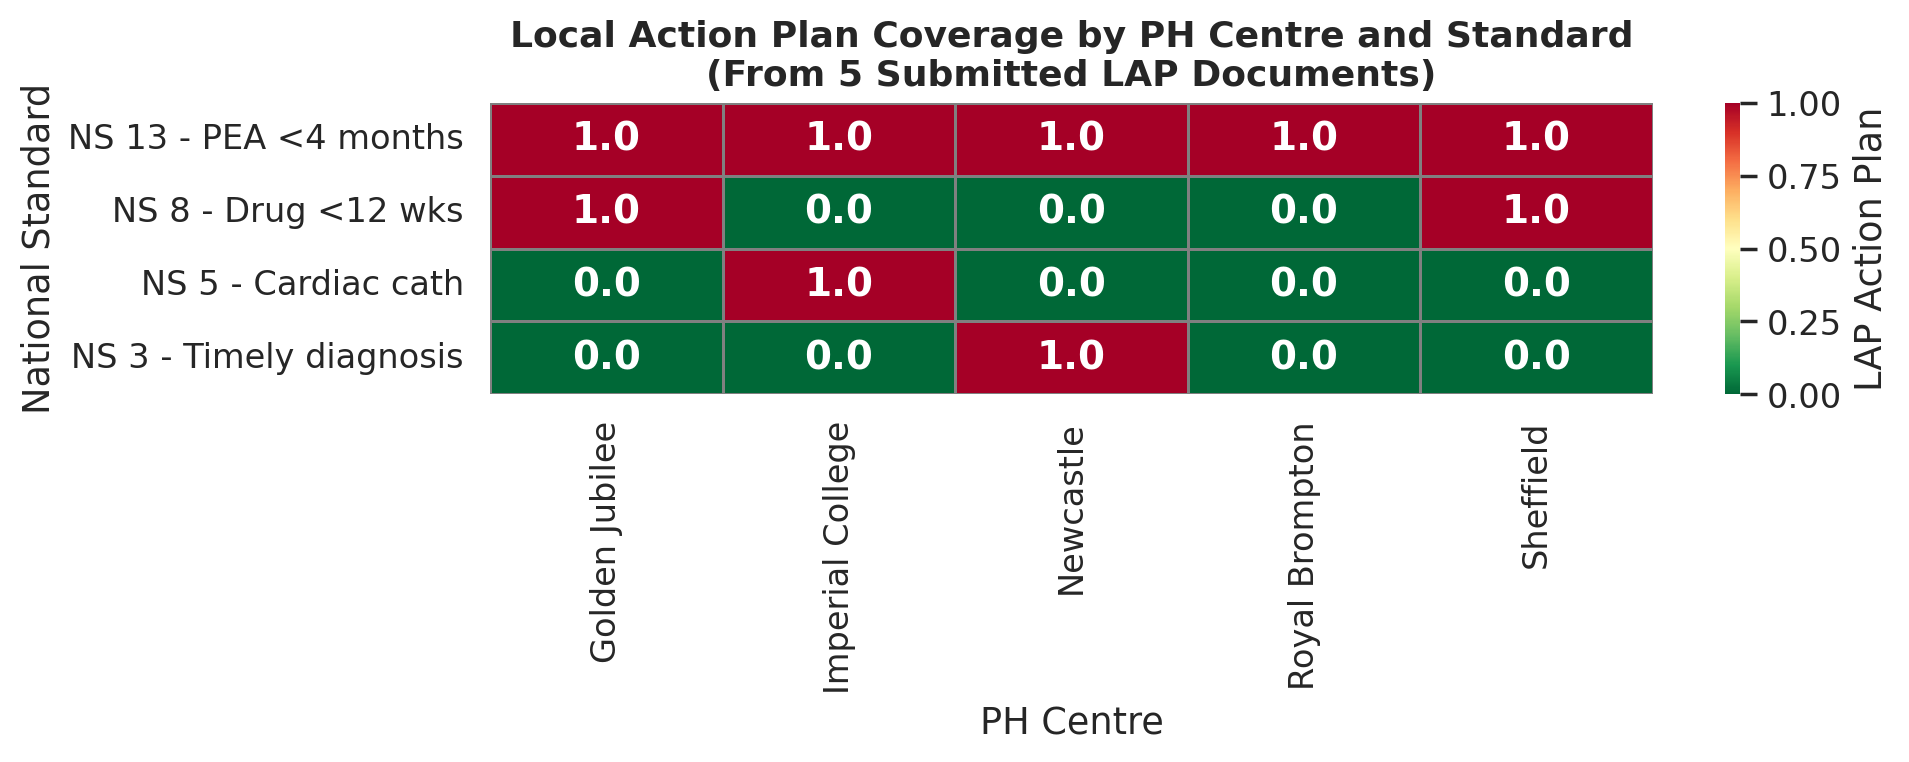
\includegraphics[width=0.75\textwidth]{lap_coverage_heatmap.png}
  \caption{Heatmap of Local Action Plan coverage. Every centre addresses Standard 13 (PEA waiting times), reflecting the urgency of this gap. Standards 3, 5, and 8 each appear in only one or two centre LAPs.}
  \label{fig:lap_coverage}
\end{figure}

\subsection{Key themes in planned actions}

\textbf{Theme 1: System-level coordination for PEA pathways.} All five LAP documents reference Royal Papworth Hospital's role in pulmonary endarterectomy. The common thread across Sheffield, Royal Brompton, Newcastle, Imperial College, and Golden Jubilee is acknowledgment that improvements require joint efforts between referring centres and the national surgical centre. Sheffield has appointed an additional secretary to reduce administrative delays and dedicated nursing staff to monitor the pathway, while examining improvements to coronary angiography waiting times. Royal Brompton continues tracking patients locally, auditing non-compliant cases, and aims to adopt a proposed virtual MDT with Royal Papworth to shorten decision timelines.

\textbf{Theme 2: Staff capacity and dedicated tracking roles.} Two centres explicitly link staffing shortages to Standard 8 failures. Sheffield reported declining performance (87\% in 2016--17 to 79\% in 2018--19) and committed to hiring a dedicated tracking member plus appointing an additional medical consultant in October 2019. Golden Jubilee aims to increase right heart catheterisation throughput and expresses optimism about meeting the standard by the 11th report cycle.

\textbf{Theme 3: Database accuracy corrections.} Imperial College identified a documentation error rather than a clinical gap: patients had undergone cardiac catheterization, but it was performed externally and the records were missing from the NAPH database. Their corrective strategy involves quarterly reviews to catch discrepancies closer to the entry date. If confirmed, this finding suggests that the true compliance rate for NS 5 may already exceed 95\%.

\textbf{Theme 4: Diagnosis documentation processes.} Newcastle (Freeman Hospital) implemented monitoring of new patient activity to ensure diagnoses are recorded within the recognised timeframe and accurately represented in the database. This is the only centre to submit a standalone LAP addressing Standard 3 (timely diagnosis), despite 94\% performance still falling below the 95\% target.

\subsection{Assessment of action plan completeness}

The submitted LAP documents exhibit notable gaps. Great Ormond Street (children's centre) did not submit a LAP document. Several centres that underperformed on national standards did not submit standalone LAP documents addressing their primary shortcomings:

\begin{itemize}[nosep]
    \item Royal Brompton submitted a LAP covering only NS 13, leaving its Standard 10 shortfall (84\% vs.\ 80\% target) unaddressed in writing.
    \item Golden Jubilee's LAP covers NS 8 and NS 13 but does not address other areas of potential improvement.
    \item Newcastle's LAP covers NS 3 and NS 13 but omits discussion of its broader service expansion efforts.
\end{itemize}

This inconsistent engagement with the Local Action Plan process limits the Audit's ability to drive measurable improvement at the centre level. A mandatory, structured LAP framework with defined scope and submission deadlines could strengthen the feedback loop between audit findings and centre-level improvement.

\section{Treatment patterns}

\subsection{Therapy escalation correlates with clinical severity}

Patients with IPAH without comorbidities receive more intensive combination therapy than those with comorbidities:

\begin{table}[H]
\centering
\small
\caption{Latest recorded therapy type by sex and IPAH type (2009--19 longitudinal cohort)}
\begin{tabularx}{\textwidth}{lrrrrY}
\toprule
Group & Total & Mono-therapy & Dual therapy & Triple+ therapy & No therapy \\
\midrule
Females (no comorbidities) & 740 & 242 (33\%) & 388 (52\%) & 86 (12\%) & 24 (3\%) \\
Males (no comorbidities) & 392 & 149 (38\%) & 192 (49\%) & 34 (9\%) & 17 (4\%) \\
Females (with comorbidities) & 204 & 112 (55\%) & 84 (41\%) & 4 (2\%) & 4 (2\%) \\
Males (with comorbidities) & 181 & 102 (56\%) & 76 (42\%) & 1 (1\%) & 2 (1\%) \\
\bottomrule
\end{tabularx}
\end{table}

Patients with comorbidities receive predominantly mono-therapy (55--56\%), likely because underlying cardiac or respiratory conditions complicate PAH-directed treatment decisions. Conversely, 64\% of women without comorbidities receive dual or triple therapy, reflecting more straightforward indications for treatment intensification.

\subsection{First-line therapy preferences}

Nationally, 91\% of patients initiate PDE5 inhibitor therapy as first-line treatment, exceeding the 80\% target. This exceeds previous years' performance (93\% in 2017--18). At the centre level, Imperial College achieves 100\%, while Royal Brompton lags at 84\%.

\section{Haemodynamic and functional profile summary}

Patients entering the longitudinal cohort present with characteristic haemodynamic profiles consistent with pre-capillary pulmonary hypertension:

\begin{table}[H]
\centering
\small
\caption{Key haemodynamic and functional parameters by sex and IPAH type}
\begin{tabularx}{\textwidth}{lcccccY}
\toprule
Parameter & Normal range & Females (no comorbidities) & Males (no comorbidities) & Females (with comorbidities) & Males (with comorbidities) & Interpretation \\
\midrule
Mean PAP (mmHg) & $<$14 (normal); $>$25 (PH) & 52.3 $\pm$ 13.1 & 49.2 $\pm$ 11.8 & 51.7 $\pm$ 10.1 & 49.2 $\pm$ 9.1 & Moderate-severe PH across all groups \\
Mean PWP (mmHg) & $<$8 & 9.7 $\pm$ 4.5 & 10.1 $\pm$ 4.8 & 12.3 $\pm$ 5.3 & 11.8 $\pm$ 4.7 & Pre-capillary pattern confirmed \\
Mean RAP (mmHg) & 0--7 & 10.0 $\pm$ 5.8 & 9.4 $\pm$ 5.4 & 12.3 $\pm$ 6.0 & 12.1 $\pm$ 6.0 & Elevated right-sided pressures \\
PVR (Wood units) & 2.5--4.2 & 12.6 $\pm$ 6.3 & 10.3 $\pm$ 4.6 & 11.2 $\pm$ 5.4 & 9.5 $\pm$ 3.9 & Markedly elevated vascular resistance \\
Six-minute walk (m) & --- & 247 $\pm$ 151 & 230 $\pm$ 152 & * & * & Limited exercise tolerance \\
emPHasis-10 score & 0--50 (0=best) & 29.1 $\pm$ 13.5 & 30.1 $\pm$ 12.9 & 31.8 $\pm$ 11.3 & * & Moderately impaired QoL \\
Cardiac index (L/m$^2$) & 2.5--4.2 & 2.2 $\pm$ 0.8 & 2.2 $\pm$ 0.7 & 2.3 $\pm$ 0.8 & 2.2 $\pm$ 0.6 & Reduced cardiac output \\
TLco (\% predicted) & 65--75 & 56 $\pm$ 20 & 51 $\pm$ 22 & 36 $\pm$ 20 & 36 $\pm$ 15 & Markedly reduced gas exchange in comorbidities \\
\bottomrule
\end{tabularx}
\end{table}

* Insufficient values to produce robust calculation ($<$50 patients).

These values cluster consistently across sex groups for patients without comorbidities. Patients with comorbidities show substantially lower lung function: TLco averages 36\% predicted versus 51--56\% predicted for those without comorbidities. FEV1 is 77\% predicted for comorbidity females and 74\% for comorbidity males, versus 86\% and 81\% respectively in the non-comorbidity groups. FVC follows a similar pattern (90\% and 86\% predicted for comorbidities versus 93\% and 89\% for non-comorbidities).

\section{Implications and recommended next steps}

\subsection{Immediate priorities}

\textbf{PEA capacity expansion is the highest-impact intervention needed.} The 79-percentage-point gap between actual performance (11\%) and the 90\% target for Standard 13 demands coordinated investment in surgical slots at Royal Papworth, streamlined pre-operative assessment pathways, and potentially expanding PEA capability to additional centres. The complex multi-disciplinary nature of the patient pathway requires joint governance between NHS England commissioners, Royal Papworth Hospital surgical teams, and referring centres.

\textbf{Drug therapy initiation bottlenecks at Sheffield and Golden Jubilee need targeted resources.} Right heart catheterisation throughput should be increased at both centres, as explicitly cited in their action plans. Dedicated case management roles can help track patients through the diagnostic-to-treatment pipeline. Sheffield has committed to adding a consultant in October 2019, which should alleviate capacity constraints.

\textbf{The vasoreactivity study standard (NS 7) requires new documentation protocols.} At 57\% versus an 80\% target, this newly introduced standard reveals a systematic recording gap. Centres must determine whether patients are receiving vasoreactivity testing but the results are not being captured in NAPH, analogous to Imperial College's cardiac catheterization documentation issue.

\subsection{Longer-term strategic directions}

\textbf{Age-stratified risk communication.} Survival data show that a 32-year-old woman with IPAH without comorbidities has dramatically different prognosis than a 78-year-old man with comorbid IPAH. PH centres should develop personalised prognosis discussions incorporating these validated predictors. Shared decision-making tools grounded in these Kaplan--Meier estimates would improve transparency in treatment conversations.

\textbf{Integration of comorbidity management into treatment pathways.} Patients with comorbidities consistently underperform on survival metrics and receive less intensive PAH-specific therapy. Multi-disciplinary approaches addressing concurrent cardiac and respiratory conditions could improve outcomes in this growing subpopulation. Current mono-therapy dominance in comorbidity groups (55--56\%) may reflect appropriate caution but could also represent undertreatment if comorbid conditions are optimally managed.

\textbf{Broaden LAP submission coverage.} Only five of eight centres submitted LAP documents, and submissions covered at most two standards each. Mandating broader LAP participation would strengthen the feedback loop between audit findings and centre-level improvement.

\subsection{Limitations}

Scottish data are excluded from survival analysis. Patients submitted by Golden Jubilee (Scotland's PH centre) are pseudo-nymised and cannot be traced via ONS or National Records of Scotland. Scottish patients are excluded from survival curves and lung function analyses, potentially biasing overall estimates given that Golden Jubilee serves the entire Scottish PH population.

Survival curves are truncated when fewer than 50 patients remain, introducing right-truncation that favours apparent longer survival for younger cohorts (which have larger denominators) relative to older ones. Curves should be interpreted as conservative estimates of true survival.

Haemodynamic characteristics derive from measurements within 90 days of diagnosis; longitudinal trajectories during treatment are not captured in this report. Cross-sectional snapshots provide a useful baseline but cannot inform about response to therapy.

Local action plan participation is self-selected. Centres may self-select which standards to address in their LAPs, leading to incomplete visibility of local quality challenges. This limitation affects the reliability of centre-level improvement tracking.

\section{Methods}

This analysis draws from two primary documents published alongside the NAPH 10th Annual Report (October 2019):

\begin{enumerate}[leftmargin=*, nosep]
    \item \textbf{NAPH 10AR -- Main Report} (NHS Digital, commissioned by NHS England, supported by NHS Scotland, NHS Wales/GIG Cymru, PHA UK, and the National Pulmonary Hypertension Centres Physicians' Committee, 24 October 2019): Contains the full set of 13 National Standards, aggregated performance data by audit year (2015--16 to 2018--19) and by PH centre, patient definitions, and methodology notes.
    \item \textbf{NAPH 10AR -- Supplementary Survival Analysis} (24 October 2019): Provides Kaplan--Meier survival curves stratified by sex, age quintiles, and WHO functional class for patients with idiopathic, heritable, and anorexigen-induced PAH (IPAH) with and without comorbidities. Data cover adult patients whose first referral was on or after 1 April 2009 (the longitudinal cohort of 23,311 patients).
    \item \textbf{Five Local Action Plan documents}: From Sheffield, Royal Brompton, Newcastle, Imperial College, and Golden Jubilee. These contain centre-specific planned actions in response to national standard shortfalls.
\end{enumerate}

Surveillance methods include structured parsing of markdown-formatted tables from source documents, tabulation of key metrics across centres and years, and creation of visualisations using Python (matplotlib and seaborn). Survival curves reproduce data directly from the supplementary report; charts are designed to aid interpretation rather than independently calculate hazard statistics. All percentages are taken from official NAPH tables and rounded according to the Audit's convention (nearest whole number).

\newpage

\begin{center}
\fbox{\parbox{0.95\textwidth}{
\centering
\small
This report was generated by \textbf{LAMBDA}, a data analysis agent.\\
Generated by LAMBDA: \url{https://lambda.com.ai}\\
Report date: \today
}}
\end{center}

\end{document}
